\iffalse
\documentclass[journal,12pt,twocolumn]{IEEEtran}
\usepackage{cite}
\usepackage{amsmath,amssymb,amsfonts,amsthm}
\usepackage{algorithmic}
\usepackage{graphicx}
\usepackage{textcomp}
\usepackage{xcolor}
\usepackage{txfonts}
\usepackage{listings}
\usepackage{enumitem}
\usepackage{mathtools}
\usepackage{gensymb}
\usepackage{comment}
\usepackage[breaklinks=true]{hyperref}
\usepackage{tkz-euclide}
\usepackage{braket}
\def\inputGnumericTable{}
\usepackage[latin1]{inputenc}
\usepackage{color}
\usepackage{array}
\usepackage{longtable}
\usepackage{calc}
\usepackage{multirow}
\usepackage{hhline}
\usepackage{ifthen}
\usepackage{lscape}
\usepackage{gvv} 
\usepackage{circuitikz}

\newtheorem{theorem}{Theorem}[section]
\newtheorem{problem}{Problem}
\newtheorem{proposition}{Proposition}[section]
\newtheorem{lemma}{Lemma}[section]
\newtheorem{corollary}[theorem]{Corollary}
\newtheorem{example}{Example}[section]
\newtheorem{definition}[problem]{Definition}
\newcommand{\BEQA}{\begin{eqnarray}}
\newcommand{\EEQA}{\end{eqnarray}}
\newcommand{\define}{\stackrel{\triangle}{=}}
\theoremstyle{remark}
\newtheorem{rem}{Remark}

\begin{document}

\bibliographystyle{IEEEtran}
\vspace{3cm}

\title{GATE 2022 IN-56}
\author{EE23BTECH11201 - Abburi Tanusha$^{*}$% <-this % stops a space
}
\maketitle
\newpage
\bigskip

\renewcommand{\thefigure}{\theenumi}
\renewcommand{\thetable}{\theenumi}

\vspace{3cm}

\maketitle
\textbf{Question:} 
The circuit shown is driven by a sinusoidal input voltage, $V_{\text{in}}$, resulting in the output voltage $V_{\text{out}}$. The frequency (in kilohertz) at which the voltage gain is 0 dB is (rounded off to two decimal places).
\begin{figure}[htb]
	\centering
	
\begin{circuitikz}
\tikzstyle{every node}=[font=\Large]
\draw [](10,10.5) to[short] (10,12.75);
\draw [](12.5,10.5) to[short] (12.5,12.75);
\draw (10,12.75) to[C] (12.5,12.75);
\draw (10.625,8.5) node[ieeestd buffer port, anchor=in](port){} (port.out) to[short] (12.25,8.5); \draw (port.in) to[short] (10.5,8.5);
\draw [](12.25,8.5) to[short, -o] (14.5,8.5);
\draw [](12.5,10.5) to[short] (12.5,8.5);
\draw [](11.25,9.75) to[short] (11.25,8.75);
\draw [](11.25,8.25) to[short] (11.25,7);
\draw [short] (10.75,8.5) -- (8.5,8.5);
\draw[] (11,8.25) to[short] (10,8.25);
\draw (10,8.25) to (10,7.25) node[ground]{};
\draw [](10,10.5) to[short] (10,8.5);
\draw (7,8.5) to[sinusoidal voltage source, sources/symbol/rotate=auto,l={ \LARGE $Vin$}] (7,6);
\draw (7,6) to (7,5.75) node[ground]{};
\node [font=\Large] at (11,13.5) {1 nF};
\node [font=\Large] at (5.75,7.25) {};
\node [font=\Large] at (15,8) {Vout};
\node [font=\Large] at (11.5,7.25) {-};
\node [font=\Large] at (11.5,9.75) {+};
\draw (10,10.75) to[R,l={ \Large $100k$}] (12.5,10.75);
\draw (7,8.5) to[R,l={ \Large $10k$}] (8.5,8.5);
\end{circuitikz}


\end{figure}
\hfill(GATE IN 2022)\\
\textbf{Solution:} 
\fi

This circuit is an inverting OP-AMP. The transfer function of an inverting OP-AMP is given by\\
\begin{table}[h]
 	\centering
 	\resizebox{14 cm}{!}{
 		
\begin{tabular}{|c|c|c|}
\hline
\textbf{Parameter} &  \textbf{Value} & \textbf{Description} \\
\hline
 $20 \log \brak{\frac{V_{\text{out}}}{V_{\text{in}}}}$ & $0$ &Voltage gain\\
\hline
 Sinusoidal input voltage & $V_{\text{in}}$ & Input voltage applied to the circuit \\
\hline
 Output voltage & $V_{\text{out}}$ & Voltage across the output of the circuit \\
\hline
$R_1$ & 10 k$\Omega$ & Resistor connected to the inverting input of the OP-AMP \\
\hline
$R_2$ & 100 k$\Omega$ & Feedback resistor connected from the output to the inverting input of the OP-AMP \\
\hline
$C$ & 1 nF & Capacitor connected in parallel with $R_2$ \\
 \hline
 $Z_1$ &  ? & Impedance of resistor $R_1$ \\
 \hline
$Z_2$ & ? & Impedance of capacitor $C$ in series with resistor $R_2$ \\
\hline
\end{tabular}



 	}
 	\vspace{6 pt}
 	\caption{Parameters}
 \end{table}
\begin{align}
Z_1 &= R_1 \\
Z_2 &= \frac{R_2}{1+j \omega R_2C} \\
\frac{1}{Z_2} &= \frac{1}{R_2} + j\omega C \\
\frac{V_{\text{out}}}{V_{\text{in}}} &= -\frac{Z_2}{Z_1} \\
\frac{|V_{\text{out}}|}{|V_{\text{in}}|} &= \frac{|Z_2|}{|Z_1|} 
\end{align}
\begin{align}
20 \log \brak{\frac{V_{\text{out}}}{V_{\text{in}}}} &= 0 \\
\frac{V_{\text{out}}}{V_{\text{in}}} &= 1
\end{align}

\begin{align}
\frac{|V_{\text{out}}|}{|V_{\text{in}}|} &= \frac{|R_2|}{|(1+ j\omega R_2C)R_1|} = 1 \\
\frac{R_2}{R_1} &= \sqrt{1 + \brak{R_2 \omega C}^2} \\
10 &= \sqrt{1 + \brak{10^5 \cdot \omega 10^-9}^2} \\
99 &= \omega^2 \times 10^{-8} \\
\omega &= \sqrt{99} \times 10^4 \\
2\pi f &= 99.49 \times 10^3 \\
f &= 15.84 \, \text{kHz}
\end{align}
\begin{figure}[h!]
\centering
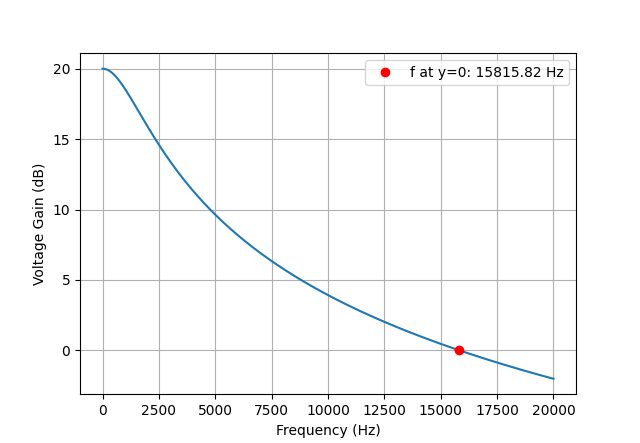
\includegraphics[width=\columnwidth]{2022/IN/56/figs/plot.png}
\caption{Frequency vs Voltage gain}
\end{figure}

%\end{document}
